\section{Evaluation}
\label{sec:eval}

We deploy our GPU code on a consumer Nvidia GeForce GTX 1060\footnote{We use the Driver Version 572.42 and CUDA Toolkit 12.8 inside WSL2 (Ubuntu 22.04 jammy).} with 6GB GDDR5. Every code change related to the GPU code is verified by comparing the resulting binary edge weights file with the one generated by our parallelized Rust implementation on the CPU. This baseline helps to quickly identify errors, which could otherwise remain unnoticed. During our tests, we define a manual threshold to cap the number of words to a user-defined threshold. The words considered are sorted according to their frequency as we are interested in relationships between the most commonly used words.

\textbf{Performance.} A fair comparison between the CPU and GPU implementation is not possible since focus was put in optimizing the GPU code. For example, the CPU implementation currently stores the row and column number alongside the actual edge weight in RAM to be able to order the results to the row-major ordering afterwards. To give an order of magnitude, the parallelized Rust CPU implementation (without the subsequent sorting) takes around $\qty{12}{\s}$ (for 10,000 nodes), \qty{42}{\s} (for 20,000 nodes) and \qty{93}{\s} for 30,000 nodes on a 4-core Intel i7-6700 CPU. The implementation is limited to around 35,000 words when $\approx\qty{20}{\giga\byte}$ of RAM are available.

\begin{figure}[H]
    \centering
    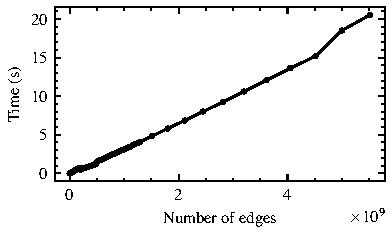
\includegraphics[width=\linewidth]{assets/timing.pdf}
    \caption{Performance of the GPU code for different number of nodes $n$. Number of edges via \eqref{eq:num-edges}.}
    \label{fig:timing}
\end{figure}

\vspace{-1.5em}

To test the performance of the GPU code, we measure the kernel execution time (including copying the results back to the host) for a range of number of nodes $n$ in the graph. For every $n$, we measure the duration 12 times\footnote{After every run, the device is re-initialized. Furthermore, we wait \qty{2}{\s} after every run before a new one starts.} and calculate mean and variance. The results are depicted in \autoref{fig:timing}. The variance is not shown as it is too small to be visible (always less than \qty{1}{\ms}). For $20,000$ words, the GPU code takes $\qty{484}{\ms}$ on average, while the CPU implementation needs $\qty{42}{\s}$. Up to $100,000$ nodes (\ie up to almost 5 billion edges), the GPU implementation takes less than \qty{20}{\s}. \autoref{fig:timing} also reveals the linear trend of time with increasing number of edges, which was to be expected since a thread is launched for every edge.

\vfill
\null


% Based on the first 100,000 most frequently used words, we calculated the distance between every pair and visualized the graph using \href{https://gephi.org/}{Gephi's} ForceAtlas2 algorithm. The neighbors of the word \q{glace} and \q{prévoir} are shown in \autoref{fig:neighbors}. For bigger graphs than that, Gephi is not able to handle the amount of data anymore.

% Having translated the problem into a graph structure also allows us to use graph algorithms to discover interesting properties. As an example, Gephi implements the \textit{shortest path algorithm}: users can click on two words and the shortest path between them is calculated and shown in the graph. Beforehand, we filtered the graph to only include the most strong edges. With this, we can find chains like the following (read them aloud to hear the phonetic similarity):
% \begin{itemize}
%     \item trottoir $\rightarrow$ entrevoir $\rightarrow$ devoir $\rightarrow$ voire $\rightarrow$ voile $\rightarrow$ val $\rightarrow$ valait $\rightarrow$ fallait $\rightarrow$ falaise
%     \item falaise $\rightarrow$ fallait $\rightarrow$ palais $\rightarrow$ passais $\rightarrow$ dépassait $\rightarrow$ dépendait $\rightarrow$ répondait $\rightarrow$ répond $\rightarrow$ raison $\rightarrow$ maison
%     \item confusion $\rightarrow$ conclusion $\rightarrow$ exclusion $\rightarrow$ explosion $\rightarrow$ exposition $\rightarrow$ explications $\rightarrow$ respiration $\rightarrow$ précipitation $\rightarrow$ présentation $\rightarrow$ présenta $\rightarrow$ présente $\rightarrow$ présence $\rightarrow$ présidence $\rightarrow$ résidence $\rightarrow$ résistance $\rightarrow$ existence
% \end{itemize}
